\section{Experimental Results}
\label{sec:experiments}

We evaluate using the two datasets. The first one is \cora dataset~\cite{mccallum-2000-cora}.  After
removing stopwords and words that appear in fewer than ten documents,
as well as documents with no words or links, our vocabulary has
1,240 unique words.  The corpus has 2,362 computer science paper abstracts
with 4,231 citation links.

The second dataset is \webkb. It is already preprocessed and has 1,703 unique words in vocabulary.
The corpus has 877 web pages with 1,608 hyperlinks.

We treat all links as undirected. Both datasets are split into 5 folds, each further split into a development and
test set with approximately the same size when used for evaluation.

\subsection{Link Prediction Results}
\label{ssec:plr}

In this section, we evaluate \lexwsbmedrtm and its variations on link
prediction tasks using \emph{predictive link rank} (\plr).  A
document's \plr is the average rank of the documents to which it has
explicit positive links, among all documents, so lower \plr is better.

Following the experiment setup in~\newcite{chang-2010-rtm}, we train the models
on the training set and predict citation links within held-out documents as well
as from held-out documents to training documents. We tune two important
parameters---$\alpha$ and negative edge ratio (the ratio of the number of
sampled negative links to the number of explicit positive links)---on the
development set and apply the trained model which performs the best on the
development set to the test set.\footnote{We also tune the number of blocks for
  embedded \wsbm and set it to 35 (\cora) and 20 (\webkb). The block topic
  priors are not applied on unseen documents, since we don't have available
  links.}  The cross validation results are given in Table~\ref{tab:plr}, where
models are differently equipped with lexical weights (\lex), \wsbm prior (\wsb),
\scc prior (\sccprefix), hinge loss (\med), and sigmoid loss
(\sigmoid).\footnote{The values of \rtm are different from the result reported
  by~\newcite{chang-2010-rtm}, because we re-preprocessed the \cora dataset and
  used different parameters.}  Link prediction generally improves with
incremental application of prior knowledge and more sophisticated learning
techniques.


\begin{table}[t!]
  \centering
  \small
  \begin{tabular}{|c|c|c|}
    \hline
    \multirow{2}{*}{\bf Model} & \multicolumn{2}{c|}{\bf \plr}\\ \cline{2-3}
     & \cora & \webkb\\ \hline
    \rtm~\cite{chang-2010-rtm} & 419.33 & 141.65\\ \hline
    \lexsccmedrtm~\cite{Yang:Boyd-Graber:Resnik-2015} & 459.55 & 150.32\\ \hhline{|=|=|=|}
    \wsbrtm & 391.88 & 127.25\\ \hline
    \lexwsbrtm & 383.25 & 125.41\\ \hline
    \lexwsbmedrtm & \bf 360.38 & \bf 111.79\\ \hline
  \end{tabular}
  \caption{Predictive Link Rank Results}\label{tab:plr}
\end{table}

The embedded \wsbm brings around 6.5\% and 10.2\% improvement over \rtm in \plr on the \cora and \webkb datasets, respectively.
This indicates that the blocks identified by \wsbm are reasonable and
consistent with reality.  The lexical weights also help link
prediction (\lexwsbrtm), though less for \wsbrtm.  This is
understandable since word distributions are much sparser and do not
make as significant a contribution as topic distributions.  Finally,
hinge loss improves \plr substantially (\lexwsbmedrtm), about 14.1\% and 21.1\% improvement over
\rtm on the \cora and \webkb datasets respectively, demonstrating the effectiveness of max-margin learning.

The only difference between \lexsccmedrtm and \lexwsbmedrtm is the
block detection algorithm.  However, their link prediction performance
is poles apart---\lexsccmedrtm even fails to outperform \rtm.  This
implies that the quality of blocks identified by \scc is not as good
as \wsbm, which we also illustrate in
Section~\ref{ssec:block_analysis}.

\subsection{Illustrative Example}
\label{ssec:illus_ex}

We illustrate our model's behavior qualitatively by looking at two abstracts,
\newcite{koplon-1997-example1} and \newcite{albertini-1992-example2} from the \cora
dataset, designated~K and~A for short.

Paper~K studies the application of Fourier-type activation functions
in fully recurrent neural networks. Paper~A shows that if two neural
networks have equal behaviors as ``black boxes", they must have the
same number of neurons and the same weights (except sign reversals).

From the titles and abstracts, we can easily find that both of them
are about \emph{neural networks} (\nn).  They both contain words like
\emph{neural}, \emph{neuron}, \emph{network}, \emph{recurrent},
\emph{activation}, and \emph{nonlinear}, which corresponds to the topic
with words \emph{neural}, \emph{network}, \emph{train}, \emph{learn},
\emph{function}, \emph{recurrent}, etc.











There is a citation between~K and~A.  The ranking of this
link improves as the model gets more sophisticated
(Table~\ref{tab:illus_plr}), except \lexsccmedrtm, which is consistent
with our \plr results.

In Figure~\ref{fig:topic_proportion}, we also show the proportions of
topics that dominate the two documents according to the various
models.  There are multiple topics dominating~K and~A according to
\rtm (Figure~\ref{fig:topic_rtm}). As the model gets more
sophisticated, the \nn topic proportion gets higher.  Finally, only
the \nn topic dominates the two documents when \lexwsbmedrtm is
applied (Figure~\ref{fig:topic_lexwsbmedrtm}).

\begin{table}[t!]
\centering
\small
\begin{tabular}{|c|c|}
  \hline
  \bf Model & \bf Rank of the Link\\ \hline
  \rtm & 1,265\\ \hline
  \lexsccmedrtm & 1,385\\ \hhline{|=|=|}
  \wsbrtm & 635\\ \hline
  \lexwsbrtm & 132\\ \hline
  \lexwsbmedrtm & \bf 106\\ \hline
\end{tabular}
\caption{\plr of the citation link between example documents~K and~A (described
  in \protect Section~\ref{ssec:illus_ex})}\label{tab:illus_plr}
\end{table}

\lexsccmedrtm gives the highest proportion to the \nn topic
(Figure~\ref{fig:topic_lexsccmedrtm}). However, the \nn topic splits into two
topics and the proportions are not assigned to the same topic, which greatly
brings down the link prediction performance. The splitting of the \nn topic also
happens in other models (Figure~\ref{fig:topic_rtm}
and~\ref{fig:topic_lexwsbrtm}), but they assign proportions to the same
topic(s). Further comparing with \lexwsbmedrtm, the blocks detected by \scc are
not improving the modeling of topics and links---some documents that should be
in two different blocks are assigned to the same one, as we will show in
Section~\ref{ssec:block_analysis}.

\begin{figure*}[ht]
\centering
\subfigure[\rtm Topic Proportions]
{
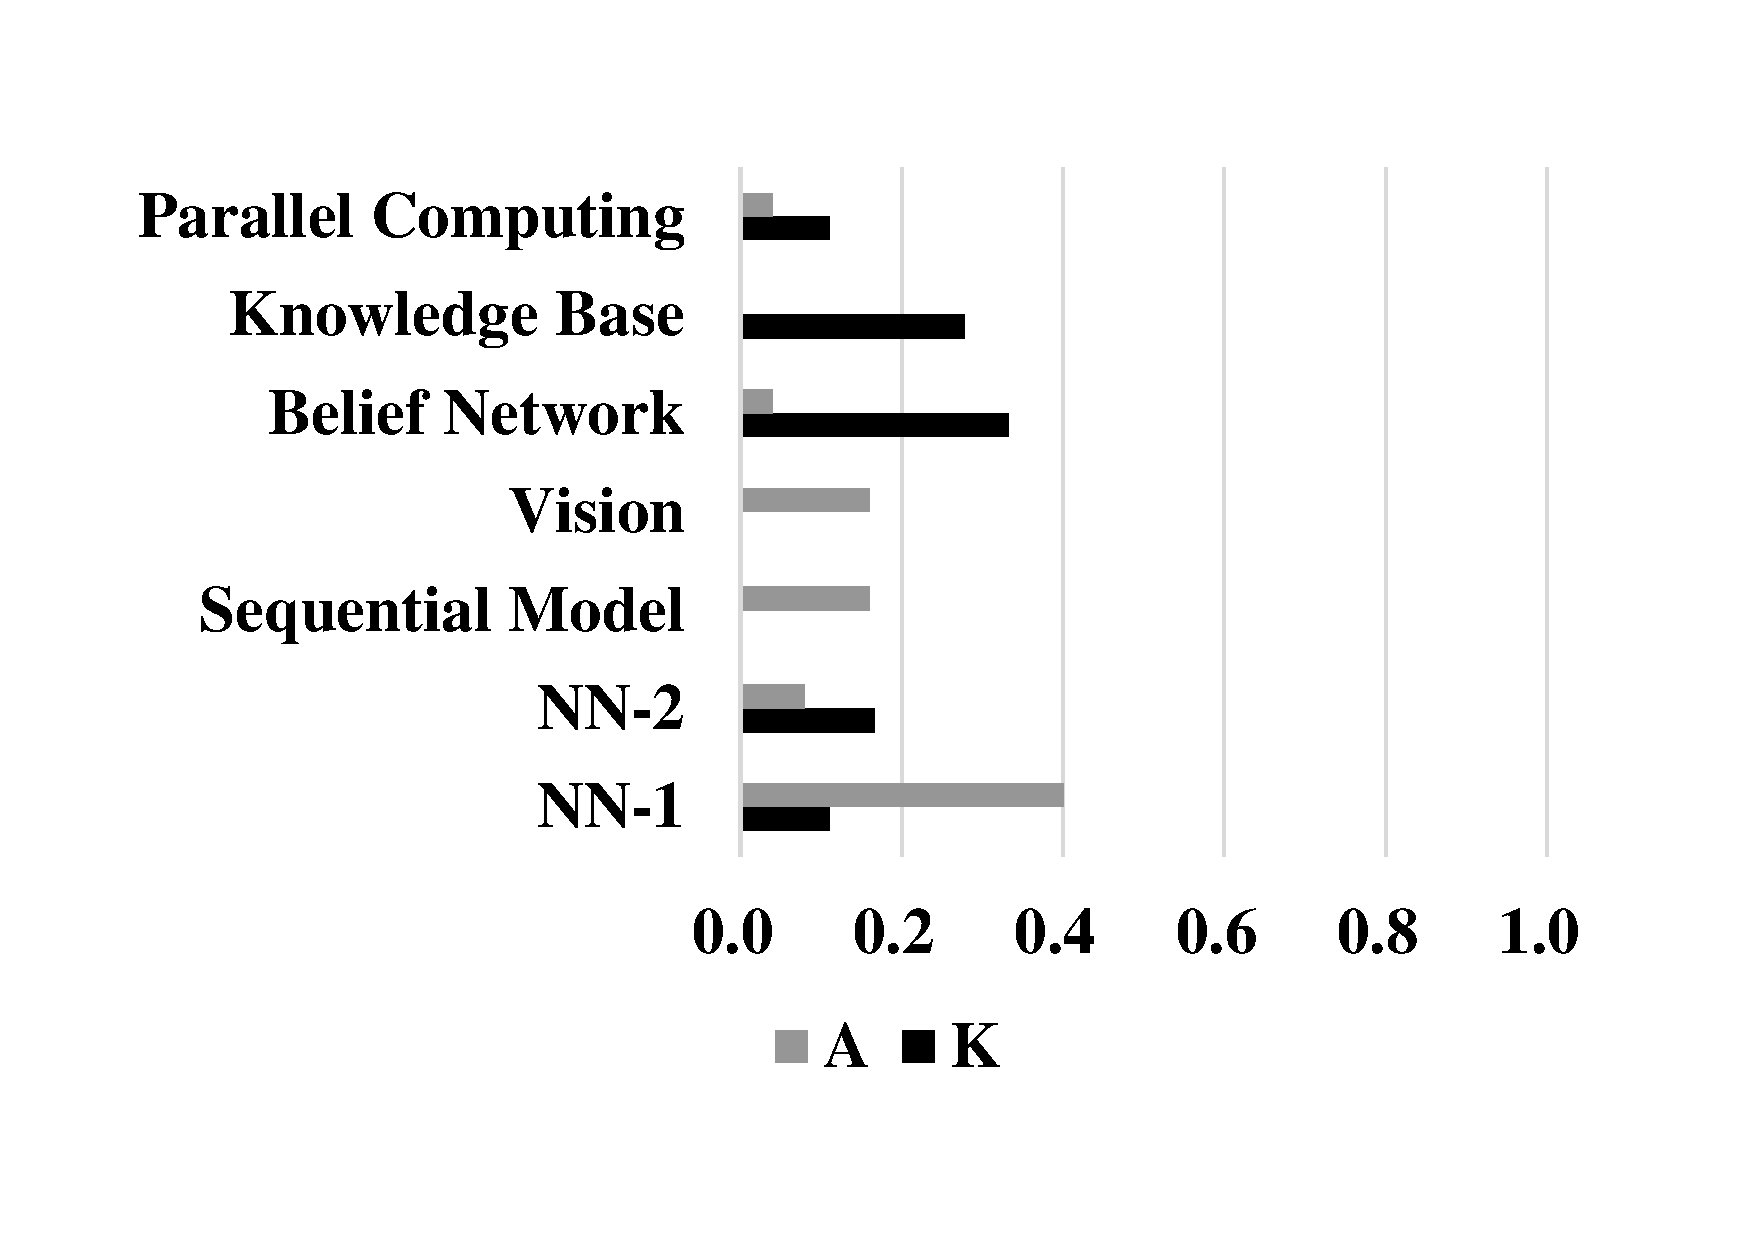
\includegraphics[width=.315\linewidth]{2016_acl_docblock/figures/topic_rtm.pdf}
\label{fig:topic_rtm}
}
\subfigure[\lexsccmedrtm Topic Proportions]
{
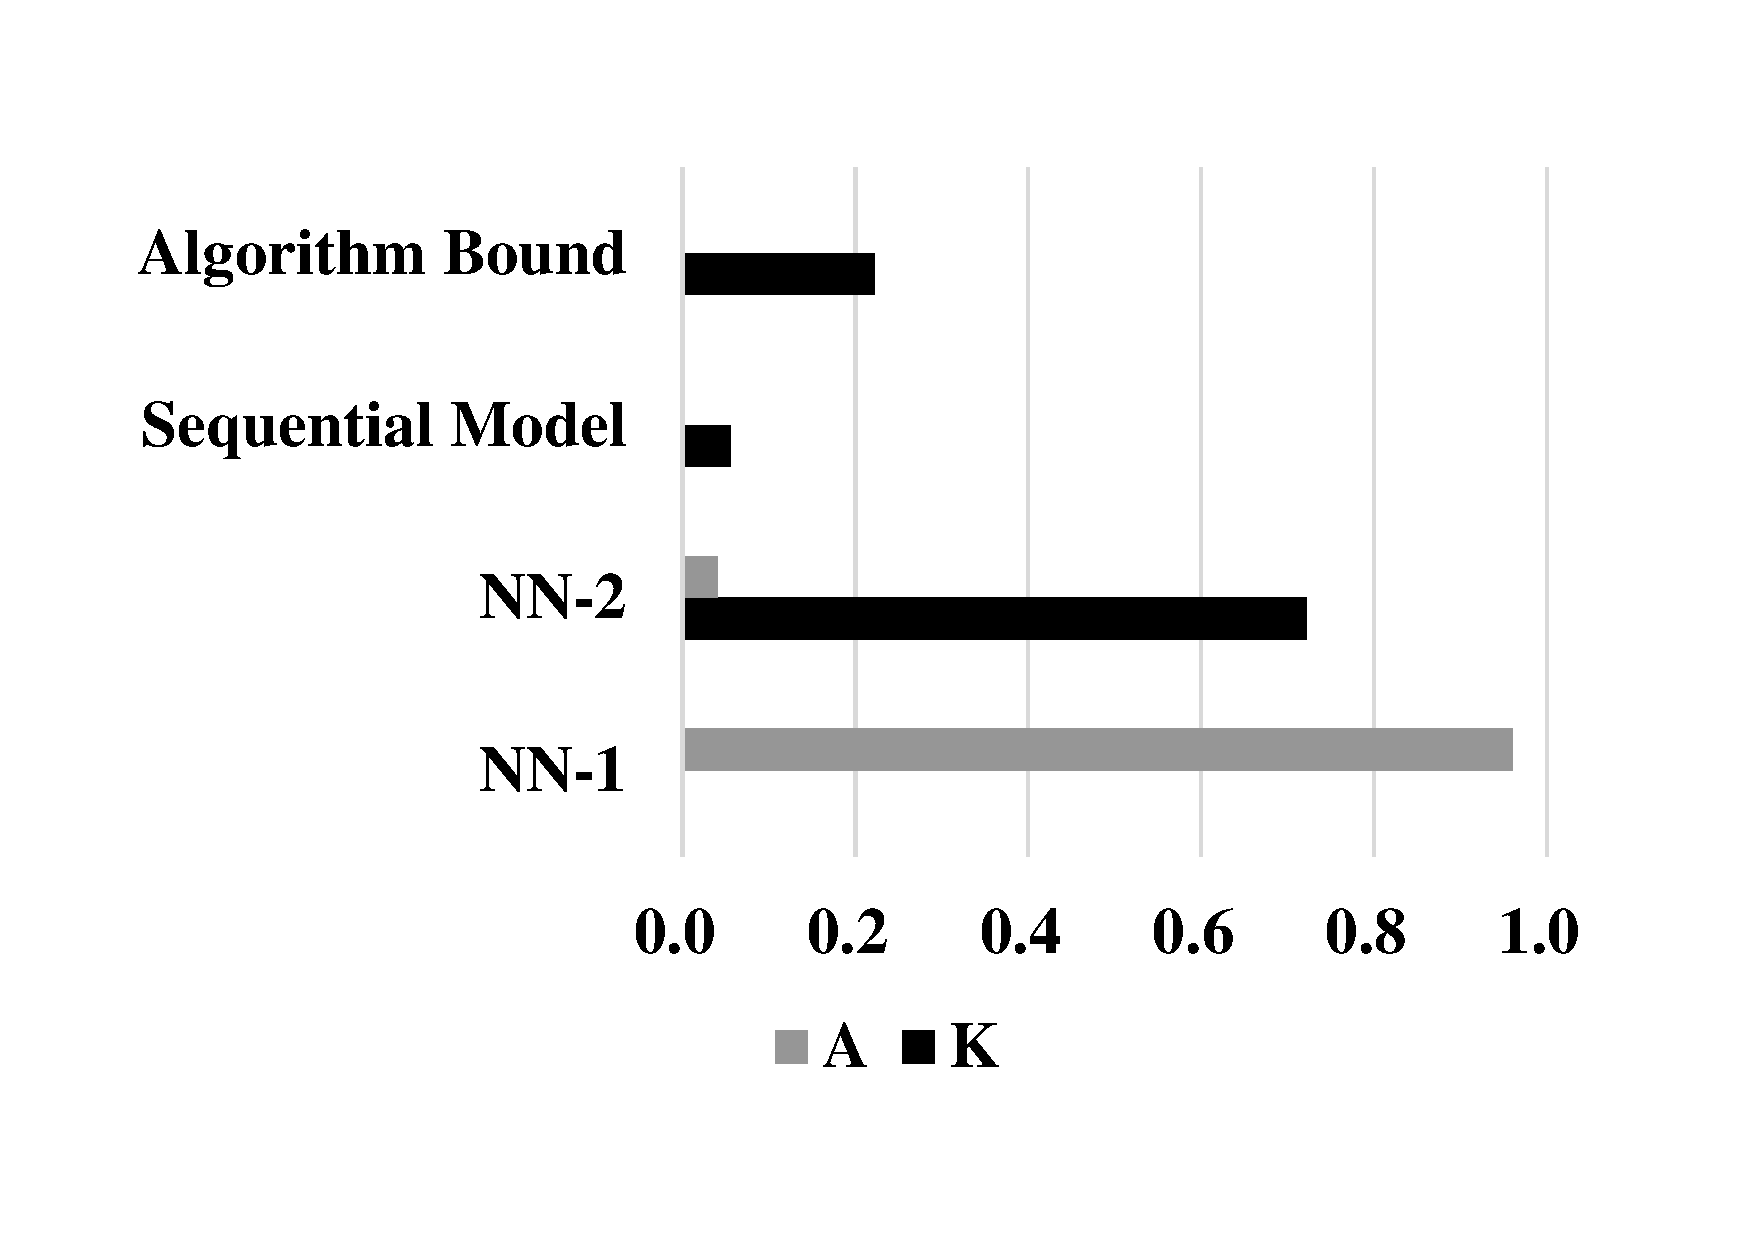
\includegraphics[width=.315\linewidth]{2016_acl_docblock/figures/topic_lexsccmedrtm.pdf}
\label{fig:topic_lexsccmedrtm}
}
\subfigure[\wsbrtm Topic Proportions]
{
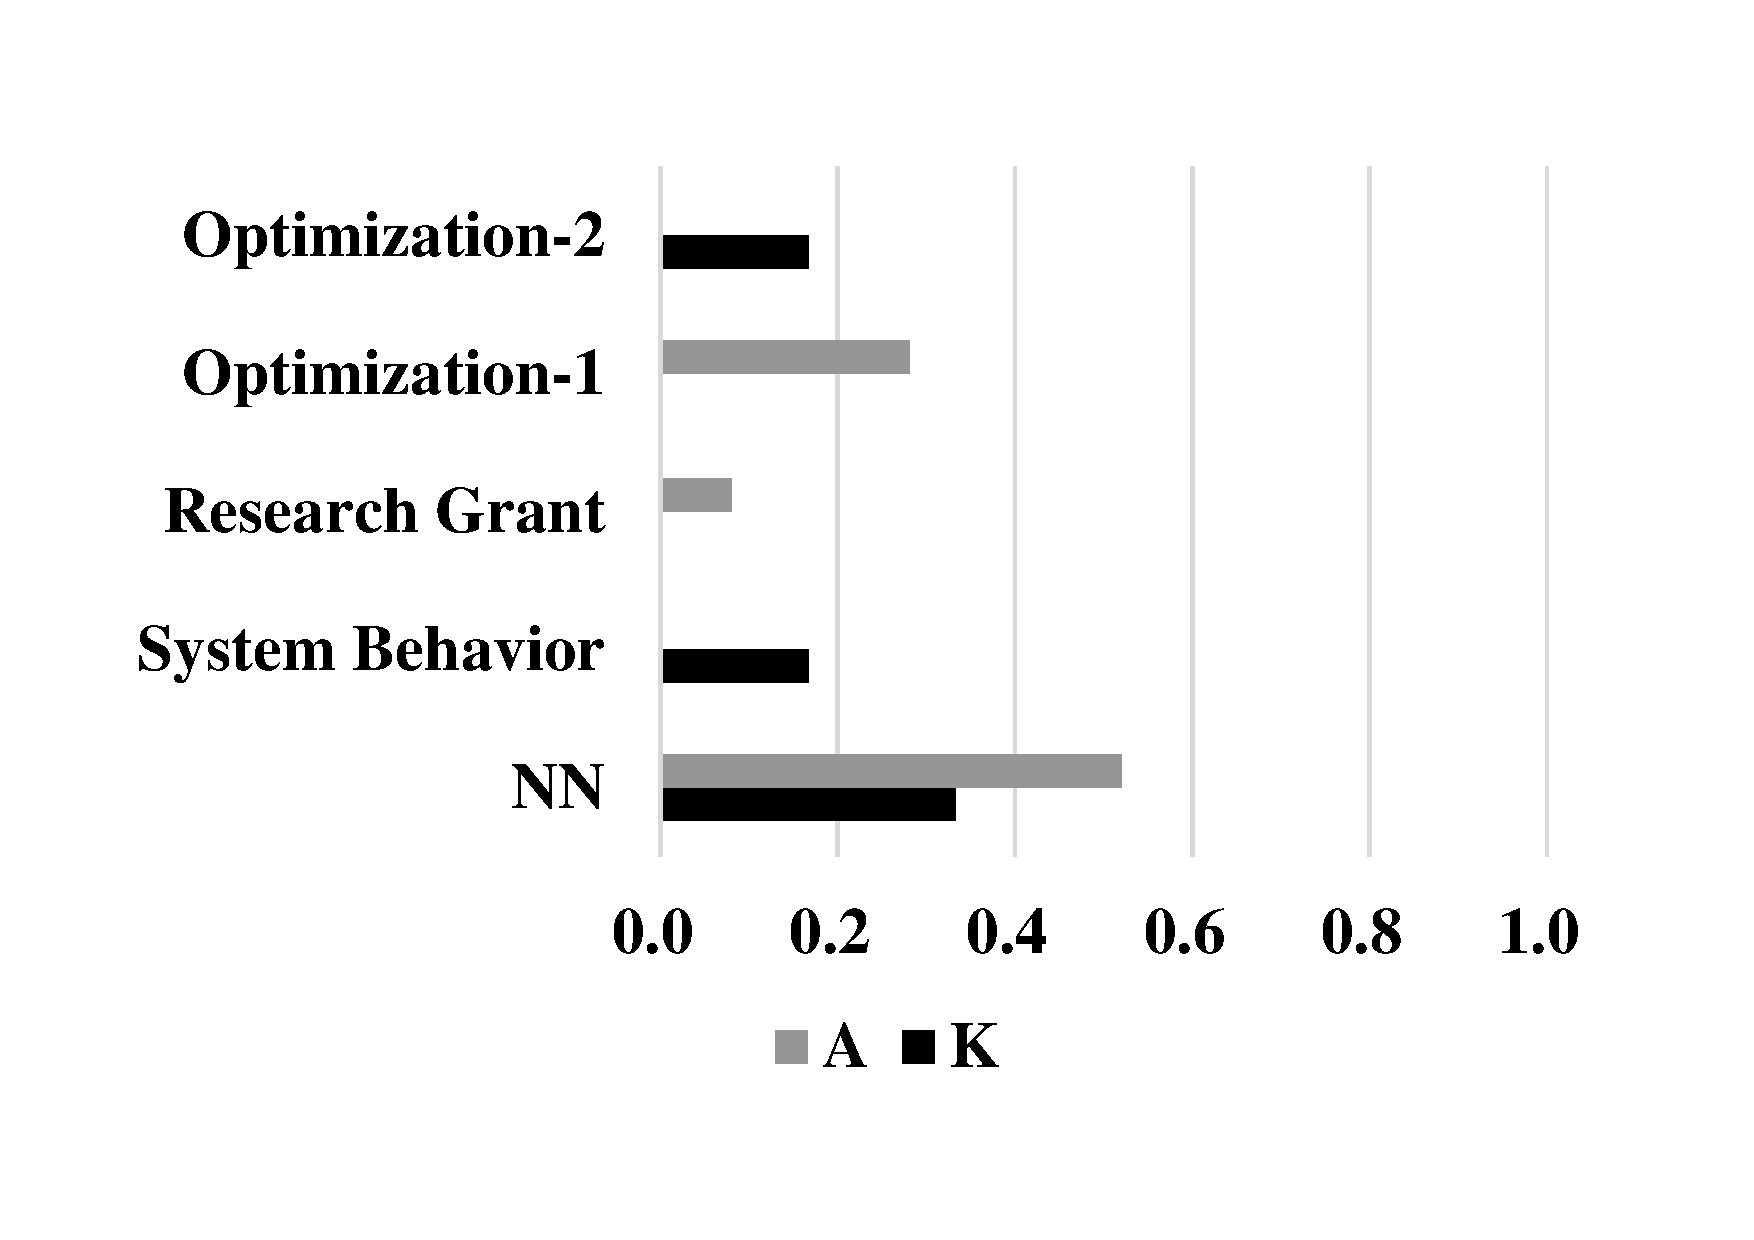
\includegraphics[width=.315\linewidth]{2016_acl_docblock/figures/topic_wsbrtm.pdf}
\label{fig:topic_wsbrtm}
}
\subfigure[\lexwsbrtm Topic Proportions]
{
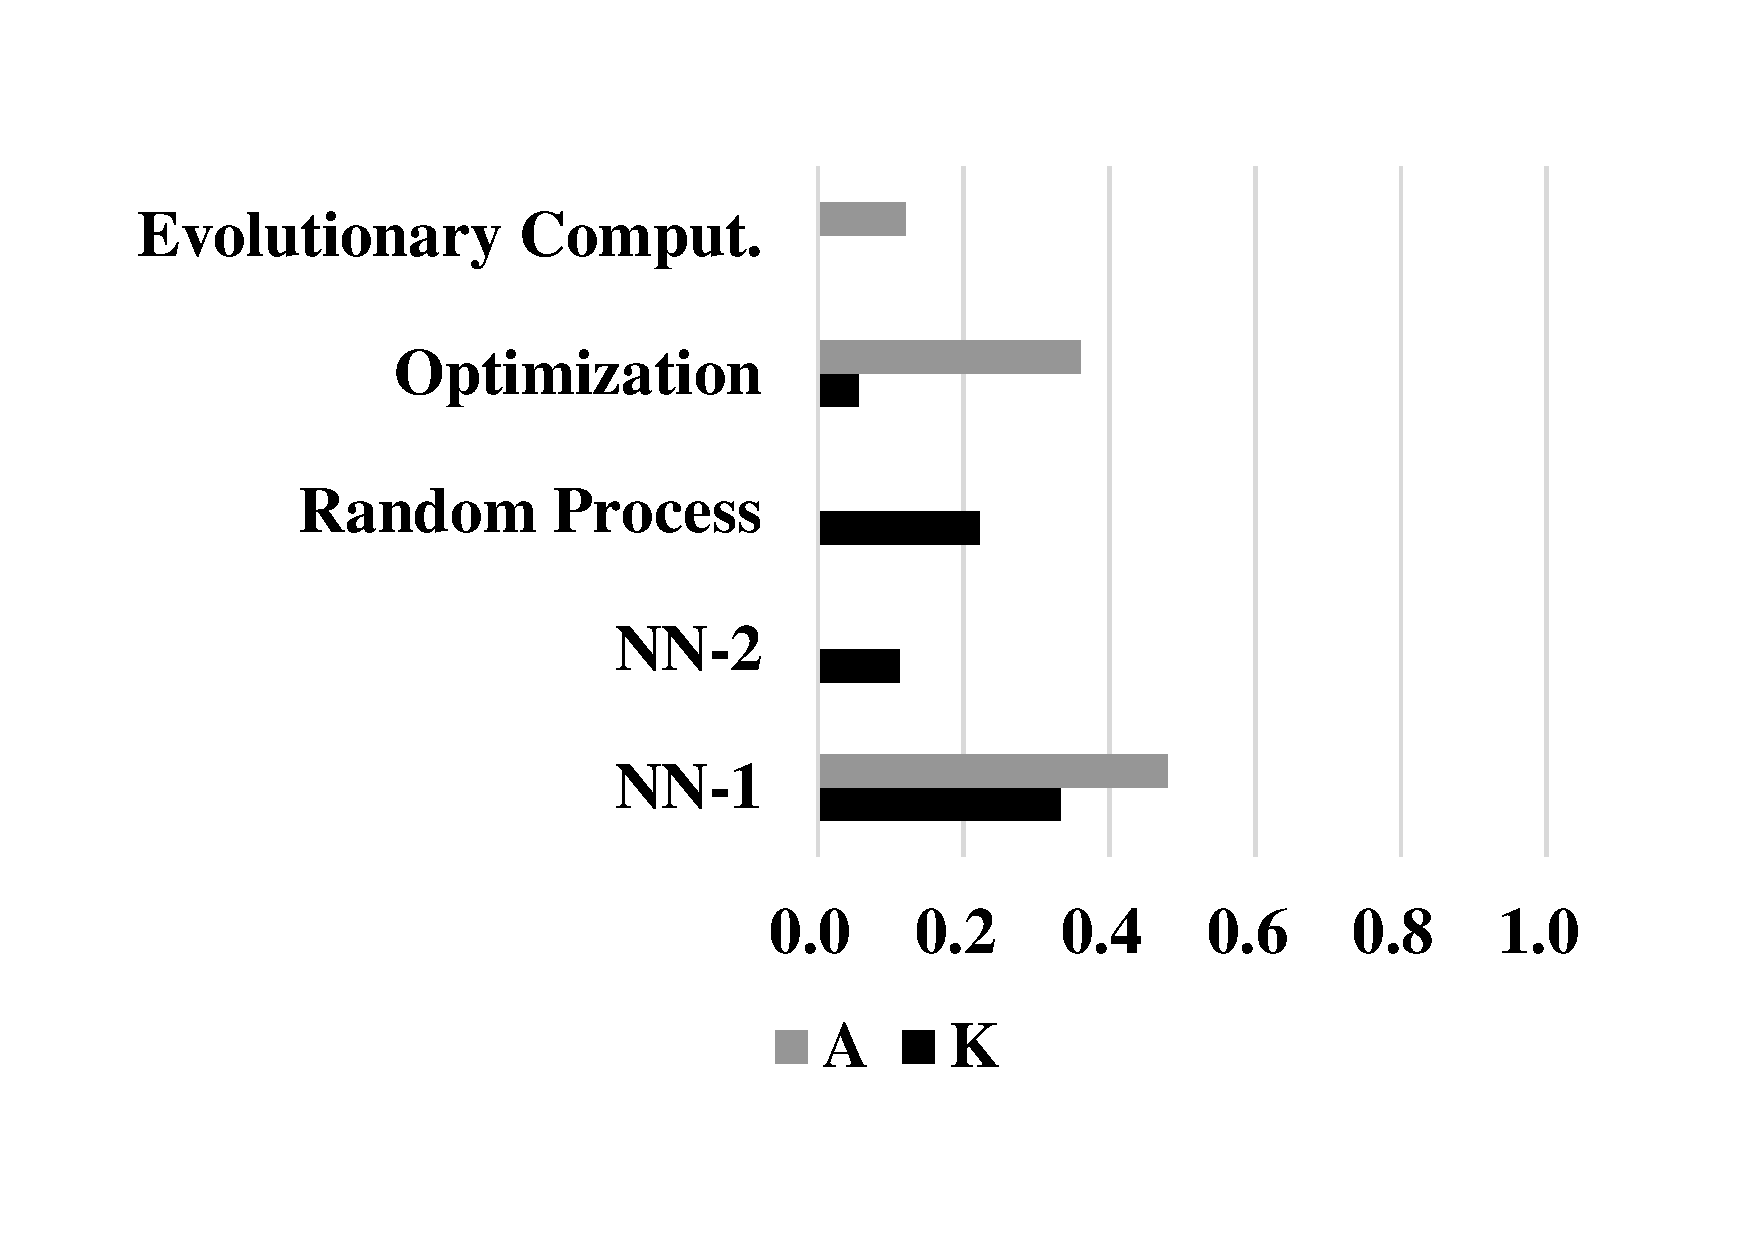
\includegraphics[width=.315\linewidth]{2016_acl_docblock/figures/topic_lexwsbrtm.pdf}
\label{fig:topic_lexwsbrtm}
}
\subfigure[\lexwsbmedrtm Topic Proportions]
{
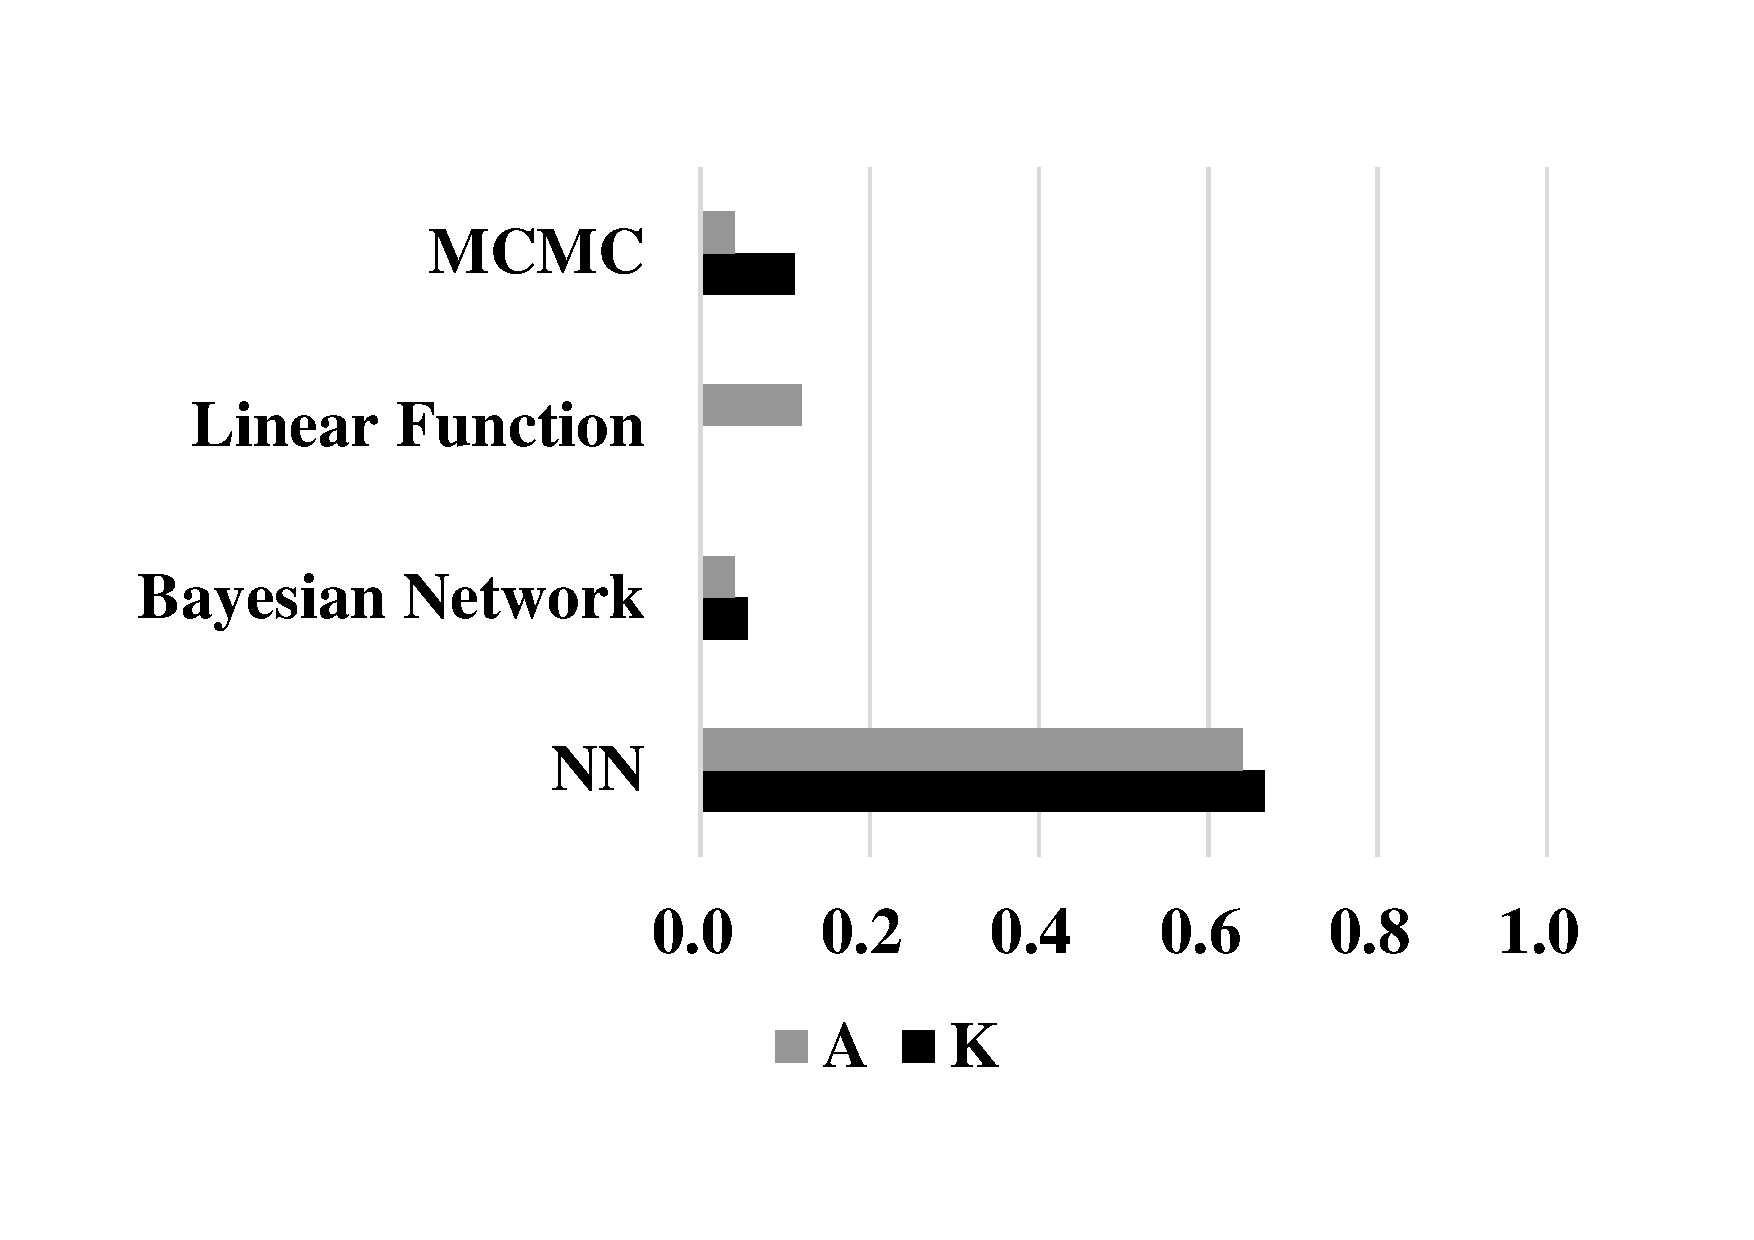
\includegraphics[width=.315\linewidth]{2016_acl_docblock/figures/topic_lexwsbmedrtm.pdf}
\label{fig:topic_lexwsbmedrtm}
}
\caption{Topic proportions given by various models on our two illustrative
  documents (K and A, described in described
  in \protect Section~\ref{ssec:illus_ex}). As the model gets more sophisticated, the \nn topic proportion gets higher and finally dominates the two documents when \lexwsbmedrtm is applied. Though \lexsccmedrtm gives the highest proportion to the \nn topic, it splits the \nn topic into two and does not assign the proportions to the same one.}\label{fig:topic_proportion}
\end{figure*}

\subsection{Topic Quality Results}
\label{ssec:topic_analysis}

We use an automatic coherence detection
method~\cite{lau-2014-auto-word-intrusion} to evaluate topic quality.
Specifically, for each topic, we pick out the top~$n$ words and
compute the average association score of each pair of words, based on
the held-out documents in development and test sets.

We choose~$n=25$ and use \emph{Fisher's exact
  test}~\cite[\fet]{upton-1992-fishers-exact-test} and \emph{log
  likelihood ratio}~\cite[\llr]{moore-2004-log-like-ratio} as the
association measures  (Table~\ref{tab:avg_assoc}).  The main advantage of these measures is that
they are robust even when the reference corpus is not large.

\begin{table}[t!]
  \centering
  \small
  \begin{tabular}{|c|c|c|c|c|}
    \hline
    \multirow{2}{*}{\bf Model} & \multicolumn{2}{c|}{\bf \fet} & \multicolumn{2}{c|}{\bf \llr}\\ \cline{2-5}
     & \bf \cora & \bf \webkb & \bf \cora & \bf \webkb\\ \hline
    \rtm & 0.1330 & 0.1312 & 3.001 & 6.055\\ \hline
    \lexsccmedrtm & 0.1418 & 0.1678 & 3.071 & 6.577\\ \hhline{|=|=|=|=|=|}
    \wsbrtm & 0.1415 & 0.1950 & 3.033 & 6.418\\ \hline
    \lexwsbrtm & 0.1342 & 0.1963 & 2.984 & 6.212\\ \hline
    \lexwsbmedrtm & \bf 0.1453 & \bf 0.2628 & \bf 3.105 & \bf 6.669\\ \hline
  \end{tabular}
  \caption{Average Association Scores of Topics}\label{tab:avg_assoc}
\end{table}

Coherence improves with \wsbm and max-margin learning, but drops a little when
adding lexical weights except the \fet score on the \webkb dataset, because lexical
weights are intended to improve link prediction performance, not topic quality.
Topic quality of \lexwsbmedrtm is also better than that of \lexsccmedrtm,
suggesting that \wsbm benefits topic quality more than \scc.

\subsection{Block Analysis}
\label{ssec:block_analysis}

In this section, we illustrate the effectiveness of the embedded \wsbm over
\scc.\footnote{We omit the comparison of \wsbm with other models, because this
  has been done by \newcite{aicher-2014-wsbm}. In addition, \wsbm is a
  probabilistic method while \scc is deterministic. They are not comparable
  quantitatively, so we compare them qualitatively.}  As we have argued, \wsbm
is able to separate two internally densely-connected blocks even if there are
few links connecting them, while \scc tends to merge them in this case.
\begin{table}[t!]
  \centering
  \small
  \begin{tabular}{|c|c|c|}
    \hline
    \bf Block & 1 & 2\\ \hline
    \bf \#Nodes & 42 & 84\\ \hline
    \bf \#Links in the Block & 55 & 142\\ \hline
    \bf \#Links across Blocks & \multicolumn{2}{c|}{2} \\ \hline
  \end{tabular}
  \caption{Statistics of Blocks 1 (learning theory) and 2 (Bayes nets), which are
    merged in \textsc{scc}.}\label{tab:block}
\end{table}
As an example, we focus on two blocks in the \cora dataset identified by \wsbm, designated
Blocks~1 and~2.  Some statistics are given in Table~\ref{tab:block}.
The two blocks are very sparsely connected, but comparatively quite
densely connected inside either block.  The two blocks' topic
distributions also reveal their differences: abstracts in Block~1
mainly focus on learning theory (\emph{learn}, \emph{algorithm},
\emph{bound}, \emph{result}, etc.) and \mcmc (\emph{markov},
\emph{chain}, \emph{distribution}, \emph{converge}, etc.).  Abstracts
in Block~2, however, have higher weights on Bayesian networks
(\emph{network}, \emph{model}, \emph{learn}, \emph{bayesian}, etc.)
and Bayesian estimation (\emph{estimate}, \emph{bayesian},
\emph{parameter}, \emph{analysis}, etc.), which differs from Block~1's
emphasis.  Because of the two inter-block links, \scc
merges the two blocks into one, which makes the block topic
distribution unclear and misleads the sampler.  \wsbm, on the other
hand, keeps the two blocks separate, which generates a high-quality
prior for the sampler.